% sizes tiny scriptsize footnotesize small normalsize large Large LARGE huge Huge

\documentclass[presentation]{beamer}

\usetheme{JuanLesPins}
\usecolortheme{orchid}
\setbeamertemplate{headline}{}
\setbeamertemplate{navigation symbols}{}

\usepackage{subfig}
\usepackage{graphicx}
\usepackage[english]{babel}
\usepackage[latin1]{inputenc}
\usepackage{color}
\usepackage{listings}
\usepackage{textcomp}
\input{listing_theme.tex}

\usepackage{tikz}
\usetikzlibrary{positioning}


% Add any additional packages you use in your presentation
% -----pack
% \usepackage{xxx}
% -----

% Add your custom definitions etc., if required
% -----misc
% \newcommand{\xxx}[1]{[#1]}
% -----




\title{Data-flow analysis}
\author[]{Michal Barczyk, Michal Cyrkowski}
\institute[]{}
\date{}


\begin{document}

\begin{frame}
  \titlepage
\end{frame}

\begin{frame}
  \frametitle{Methods of collecting context information from AST}
  
   \begin{itemize}
    \item symbolic interpretation
    \item data-flow equations
    \end{itemize}
\end{frame}

\begin{frame}
  \frametitle{Methods of collecting context information from AST}
  
%   \begin{definition}
% A prime number is a number that...
% \end{definition}

\begin{block}{Control-flow graph}
For each AST node we need to know its flow-of-control successor(s). We can represent it as an additional data structure where every node has pointer or pointers to its flow-of-control successor. Pointers can be visualised on orginal AST.
\end{block}

\begin{block}{Threading the tree}
Threading is a method of constructing control-flow graph. For each node threading routine detects production describing node and calls threading routine on its children recoursively. Each instance of threading routine is aware of global variable \emph{last\_node\_pointer} pointing to the last node processed on the controlflow
path.
\end{block}
   
\end{frame}

\begin{frame}
  \frametitle{Threading the AST}
  \begin{block}{}
    Using this technique, the threading routine for a binary expression could, for example, have the following form: 
    
    \lstinputlisting[language=Python]{procedure1.py}
    
    This makes the present node the successor of the last node of the right operand and then registers it as the next dynamically last node.
  \end{block}
  


  
\end{frame}

\begin{frame}
  \frametitle{Threading the AST}
  
   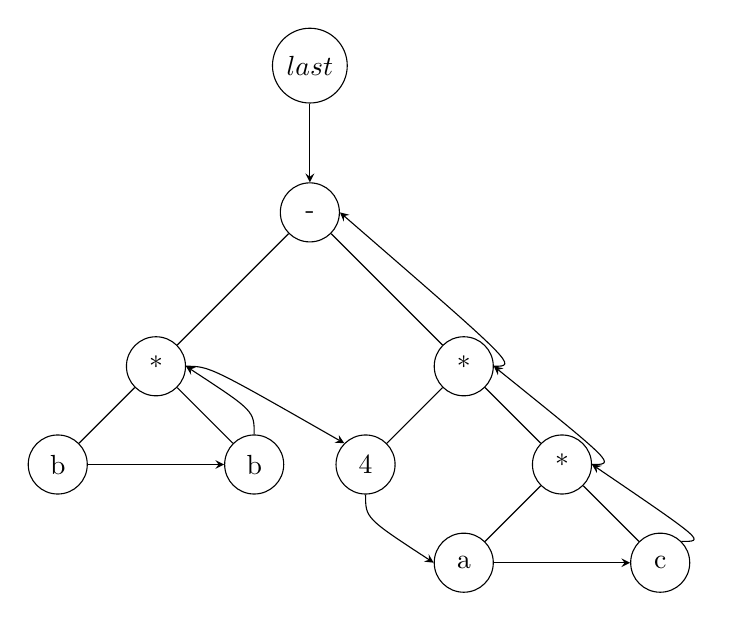
\begin{tikzpicture}[>=stealth, every node/.style={circle, draw, minimum size=0.75cm}]
   
        %Nodes
        \node   (last) {$last$};
        \node   (minus) [below=1 of last] {-};
        \node   (star1) [below left=2 of minus] {*};
        \node   (b1) [below left=1 of star1] {b};
        \node   (b2) [below right=1 of star1] {b};
        \node   (star2) [below right=2 of minus] {*};
        \node   (four) [below left=1 of star2] {4};
        \node   (star3) [below right=1 of star2] {*};
        \node   (a) [below left=1 of star3] {a};
        \node   (c) [below right=1 of star3] {c};
        
        
        % \node      (rightsquare)       [right=of maintopic] {3};
        % \node       (lowercircle)       [below=of maintopic] {4};
        
        %Lines
        \draw[-] (minus.south west) -- (star1.north east);
        \draw[-] (minus.south east) -- (star2.north west);
        \draw[-] (star1.south west) -- (b1.north east);
        \draw[-] (star1.south east) -- (b2.north west);
        \draw[-] (star2.south west) -- (four.north east);
        \draw[-] (star2.south east) -- (star3.north west);
        \draw[-] (star3.south west) -- (a.north east);
        \draw[-] (star3.south east) -- (c.north west);
        
        \draw[->] (b1.east) .. controls +(right:3mm)  .. (b2.west);
        \draw[->] (b2.north) .. controls +(up:3mm)  .. (star1.east);
        \draw[->] (star1.east) .. controls +(right:3mm)  .. (four.north west);
        \draw[->] (four.south) .. controls +(down:3mm)  .. (a.west);
        \draw[->] (a.east) .. controls +(right:3mm)  .. (c.west);
        \draw[->] (c.north east) .. controls +(right:3mm)  .. (star3.east);
        \draw[->] (star3.east) .. controls +(right:3mm)  .. (star2.east);
        \draw[->] (star2.east) .. controls +(right:3mm)  .. (minus.east);
        
        \draw[->] (last.south) .. controls +(down:3mm)  .. (minus.north);
    
    \end{tikzpicture}
  
  


\end{frame}

\begin{frame}
  \frametitle{Threading the AST}
  \begin{block}{Problems}
  The problem occurs if the flow of control exists in more than one place. The perfect example is if/else statment that causes two problems. The first is that node that corresponds to the run-time then/else decision has two successors rather than one. The second is that when we reach the node dynamically following the entire if-statement, its address must be recorded in the dynamically last nodes of both the then-part and the else-part. As a result single variable \emph{last\_node\_pointer} is no longer sufficient.
  \end{block}
  
\end{frame}

\begin{frame}
  \frametitle{Threading the AST}
  \begin{block}{First problem solution}
  This issue can be simply solved  by storing pointers to two successors in the if-node.
  \end{block}
  
  \begin{block}{Second problem solution}
  One way to solve the second problem is to replace \emph{last\_node\_pointer} by a set of last nodes that will be filled in when next node in the control-flow path is dynamically found.\\
  Another method is to construct a special join node to merge the diverging flow of control. Such node is part of control-flow graph without being part of AST.
  \end{block}
  
\end{frame}

\begin{frame}
  \frametitle{Methods of collecting context information from AST}
  
  \lstinputlisting[language=Python]{procedureIf.py}
  
\end{frame}

\begin{frame}
  \frametitle{Methods of collecting context information from AST}
  
  \begin{alertblock}{Wykres}

    \end{alertblock}
  
\end{frame}

\begin{frame}
  \frametitle{Symbolic interpretation}
  
  \begin{block}{Symbolic interpretation}
  During program execution, the control follow one possible path through the control-flow graph. The behaviour of a code block is determined by the values of the variables created/assigned before execution of this block and this block can change values of variables determining a following execution (path in control-flow graph). Much contextual information about variables can be deduced statically by
  simulating process of execution at compile
  time.This technique is called \textbf{symbolic interpretation} or simulation on the stack.
  \end{block}
  
\end{frame}

\begin{frame}
  \frametitle{Symbolic interpretation}
  \begin{block}{Stack representation in control-flow graph of if-statement}
  In this example we assume that we arrive with a stack containing two variables x and y.\\
  x is initialized and y is valued 5. The condition is y $>$ 0.
  \end{block}
  wykres
\end{frame}

\begin{frame}
  \frametitle{Simple symbolic interpretation}
  
  \begin{block}{Simple symbolic interpretation}
  \textbf{Simple symbolic interpretation} allows us to check for the use of uninitialized variables. In order to do it, we create compile-time representation of the local stack as list of pairs \emph{(name, property)}. 
  \begin{itemize}
    \item At the beginning property list is empty or contains parameters with properties since parameters are obviously initialized.
    \item Then we follow the path on control-flow graph processing encountered varibles.
    \item When a declaration is met, the declared name is added to the property list with status: initialized or uninitialized.
    
    \end{itemize}
 
  \end{block}
  
\end{frame}

\begin{frame}
  \frametitle{Simple symbolic interpretation}
  
  \begin{block}{Simple symbolic interpretation}
  \begin{itemize}
    \item When the control-flow splits (eg. if-node) there is made a copy of property list and simulated execution is done for then-part and for else-part.
    \item When an assignment is met, the status of the destination variable is set to
    initialized, after processing the source expression first, since it may contain the same
    variable.
    \item When the variable is used (eg. in expression), its status is checked in property list. If its status is uninitialized/possibly uninitialized we are given error/warning.
    \end{itemize}
 
  \end{block}
  
\end{frame}

\begin{frame}
  \frametitle{Simple symbolic interpretation}
  
  \begin{block}{Stack representations in the control-flow graph of a for loop}
  When the interpreter meets a for statement it passes through the bands and the inintalization of the controlled variable. It then makes a copy of the list which is called the \textbf{loop-exit list}. This list collects the information at the exit of the loop.\\
  \begin{itemize}
      \item If loop-exit statement is found inside the loop the callected list is merged into loop-exit list and interpretation continues with empty list.\\
      \item If return statement is found inside loop or we reach the end of the routine present list is merged into loop-exit list and interpretation sontinues with empty list.
  \end{itemize}
  \end{block}
  
\end{frame}

\begin{frame}
  \frametitle{Simple symbolic interpretation}
  \begin{block}{Stack representations in the control-flow graph of a for loop}
  \begin{itemize}
      \item If return statement is found outside loop interpreter can raise an error.
      \item If the end of the routine node is reached interpreter checks all variable identifiers in the list. If on has status \emph{Uninitialized} it never was initialized and a warning can be given.
  \end{itemize}
  \textbf{Note that the interpreter ignores the back jump of the for-statement}.
  \end{block}
  
\end{frame}

\begin{frame}
  \frametitle{Simple symbolic interpretation}
  rys 5.10
  
\end{frame}

\begin{frame}
  \frametitle{Simple symbolic interpretation}
  \begin{block}{Simple symbolic interpretation requierments}
  \begin{itemize}
      \item The program must consist of flow-of-control structures with one entry point and one exit point only.
      \item The values of the property must form a lattice, which means that the values can be ordered in a sequence $v_1...v_n$ such that there is no operation that will transform $v_j$ into $v_i$; we will write $v_i < v_j$ for all $i<j$.
      \item The result of merging two values must be at least as large as the smaller of the two.
      \item An action taken on $v_i$ in a given situation must make any action taken on $v_j$ in the same situation superfluous, for $v_i \leq v_j$.
  \end{itemize}
  \end{block}
  \begin{block}{}
  If this four requirements are not fulfilled it is necessary to preform \textbf{full symbolic interpretation} that avoids above shortcuts.
  \end{block}
\end{frame}

\begin{frame}
  \frametitle{Full symbolic interpretation}
  \begin{block}{Full symbolic interpretation}
  Goto statements cannot be handled by simple symbolic interpretation, since they
violate requirement 1 from the previous slide. In order to handle them, we use \textbf{full symbolic interpretation}. 
  
  \end{block}
  
\end{frame}

\begin{frame}
  \frametitle{Methods of collecting context information from AST}
  
\end{frame}

\begin{frame}
  \frametitle{Methods of collecting context information from AST}
  
\end{frame}

\begin{frame}
  \frametitle{Methods of collecting context information from AST}
  
\end{frame}

\begin{frame}
  \frametitle{Methods of collecting context information from AST}
  
\end{frame}

\begin{frame}
  \frametitle{Methods of collecting context information from AST}
  
\end{frame}

\begin{frame}
  \frametitle{Methods of collecting context information from AST}
  
\end{frame}

\begin{frame}
  \frametitle{Methods of collecting context information from AST}
  
\end{frame}

\begin{frame}
  \frametitle{Methods of collecting context information from AST}
  
\end{frame}

\begin{frame}
  \frametitle{Methods of collecting context information from AST}
  
\end{frame}


\end{document}
